\newpage

\subsection{Patterns}
Patterns, sogenannte Entwurfsmuster, wurden ursprünglich vom Architekten Christopher Alexander geprägt.
Dieser beschrieb in seinem Buch \enquote{A Pattern Language: Towns, Buildings, Construction}\cite{a-pattern-language} im Jahr 1977 zum ersten Mal Muster, unter dessen Einsatz sich wiederkehrende Probleme lösen lassen.
In der Informatik wurden Entwurfsmuster durch die Veröffentlichung der \enquote{Gang of Four} im Jahr 1994 populärer.
In ihrem Buch \enquote{Design Patterns - Elements of Reusable Object-Oriented Software}\cite{gamma-design-patterns} beschreiben Erich Gamma et al.\ 23 unterschiedliche Entwurfsmuster.
Diese sind eingeteilt in die drei Kategorien Creational, Structural und Behavioral.

1999 ergänzte Martin Fowler in \enquote{Patterns of Enterprise Application Architecture}\cite{patterns-of-enterprise-application-architecture} die Kategorie \enquote{Objektrelationale Abbildung} und dazugehörige Muster.
Gregor Hohpe und Bobby Woolf ergänzten 2003 die Kategorie der Messaging Patterns in ihrem Buch \enquote{Enterprise Integration Patterns}\cite{enterprise-integration-patterns}.

Die Menge der Entwurfsmuster ist sehr umfangreich, weshalb im Folgenden nur jene Muster skizziert werden, die im anschließenden Vergleich verwendet werden.

\subsubsection{MVC (Model-View-Controller)}
Dieses architektonische Pattern teilt eine interaktive Anwendung in drei Komponenten auf.
Durch eine klare Trennung der Zuständigkeiten werden Wartungen einfacher und können besser auf unterschiedliche Entwickler aufgeteilt werden.
Das Model ist nur zuständig für Daten und Business Logic, die View hingegen, nur für die Darstellung der Inhalte (\ref{fig:mvc}).
Der Controller ist das Bindeglied und routet Daten sowie Befehle zwischen den beiden anderen Bereichen.
(Vgl.~\cite{buschmann-pattern-oriented-software-architecture})

\begin{figure}[h!]
    \centering
    \caption{Model View Controller}
    \label{fig:mvc}
    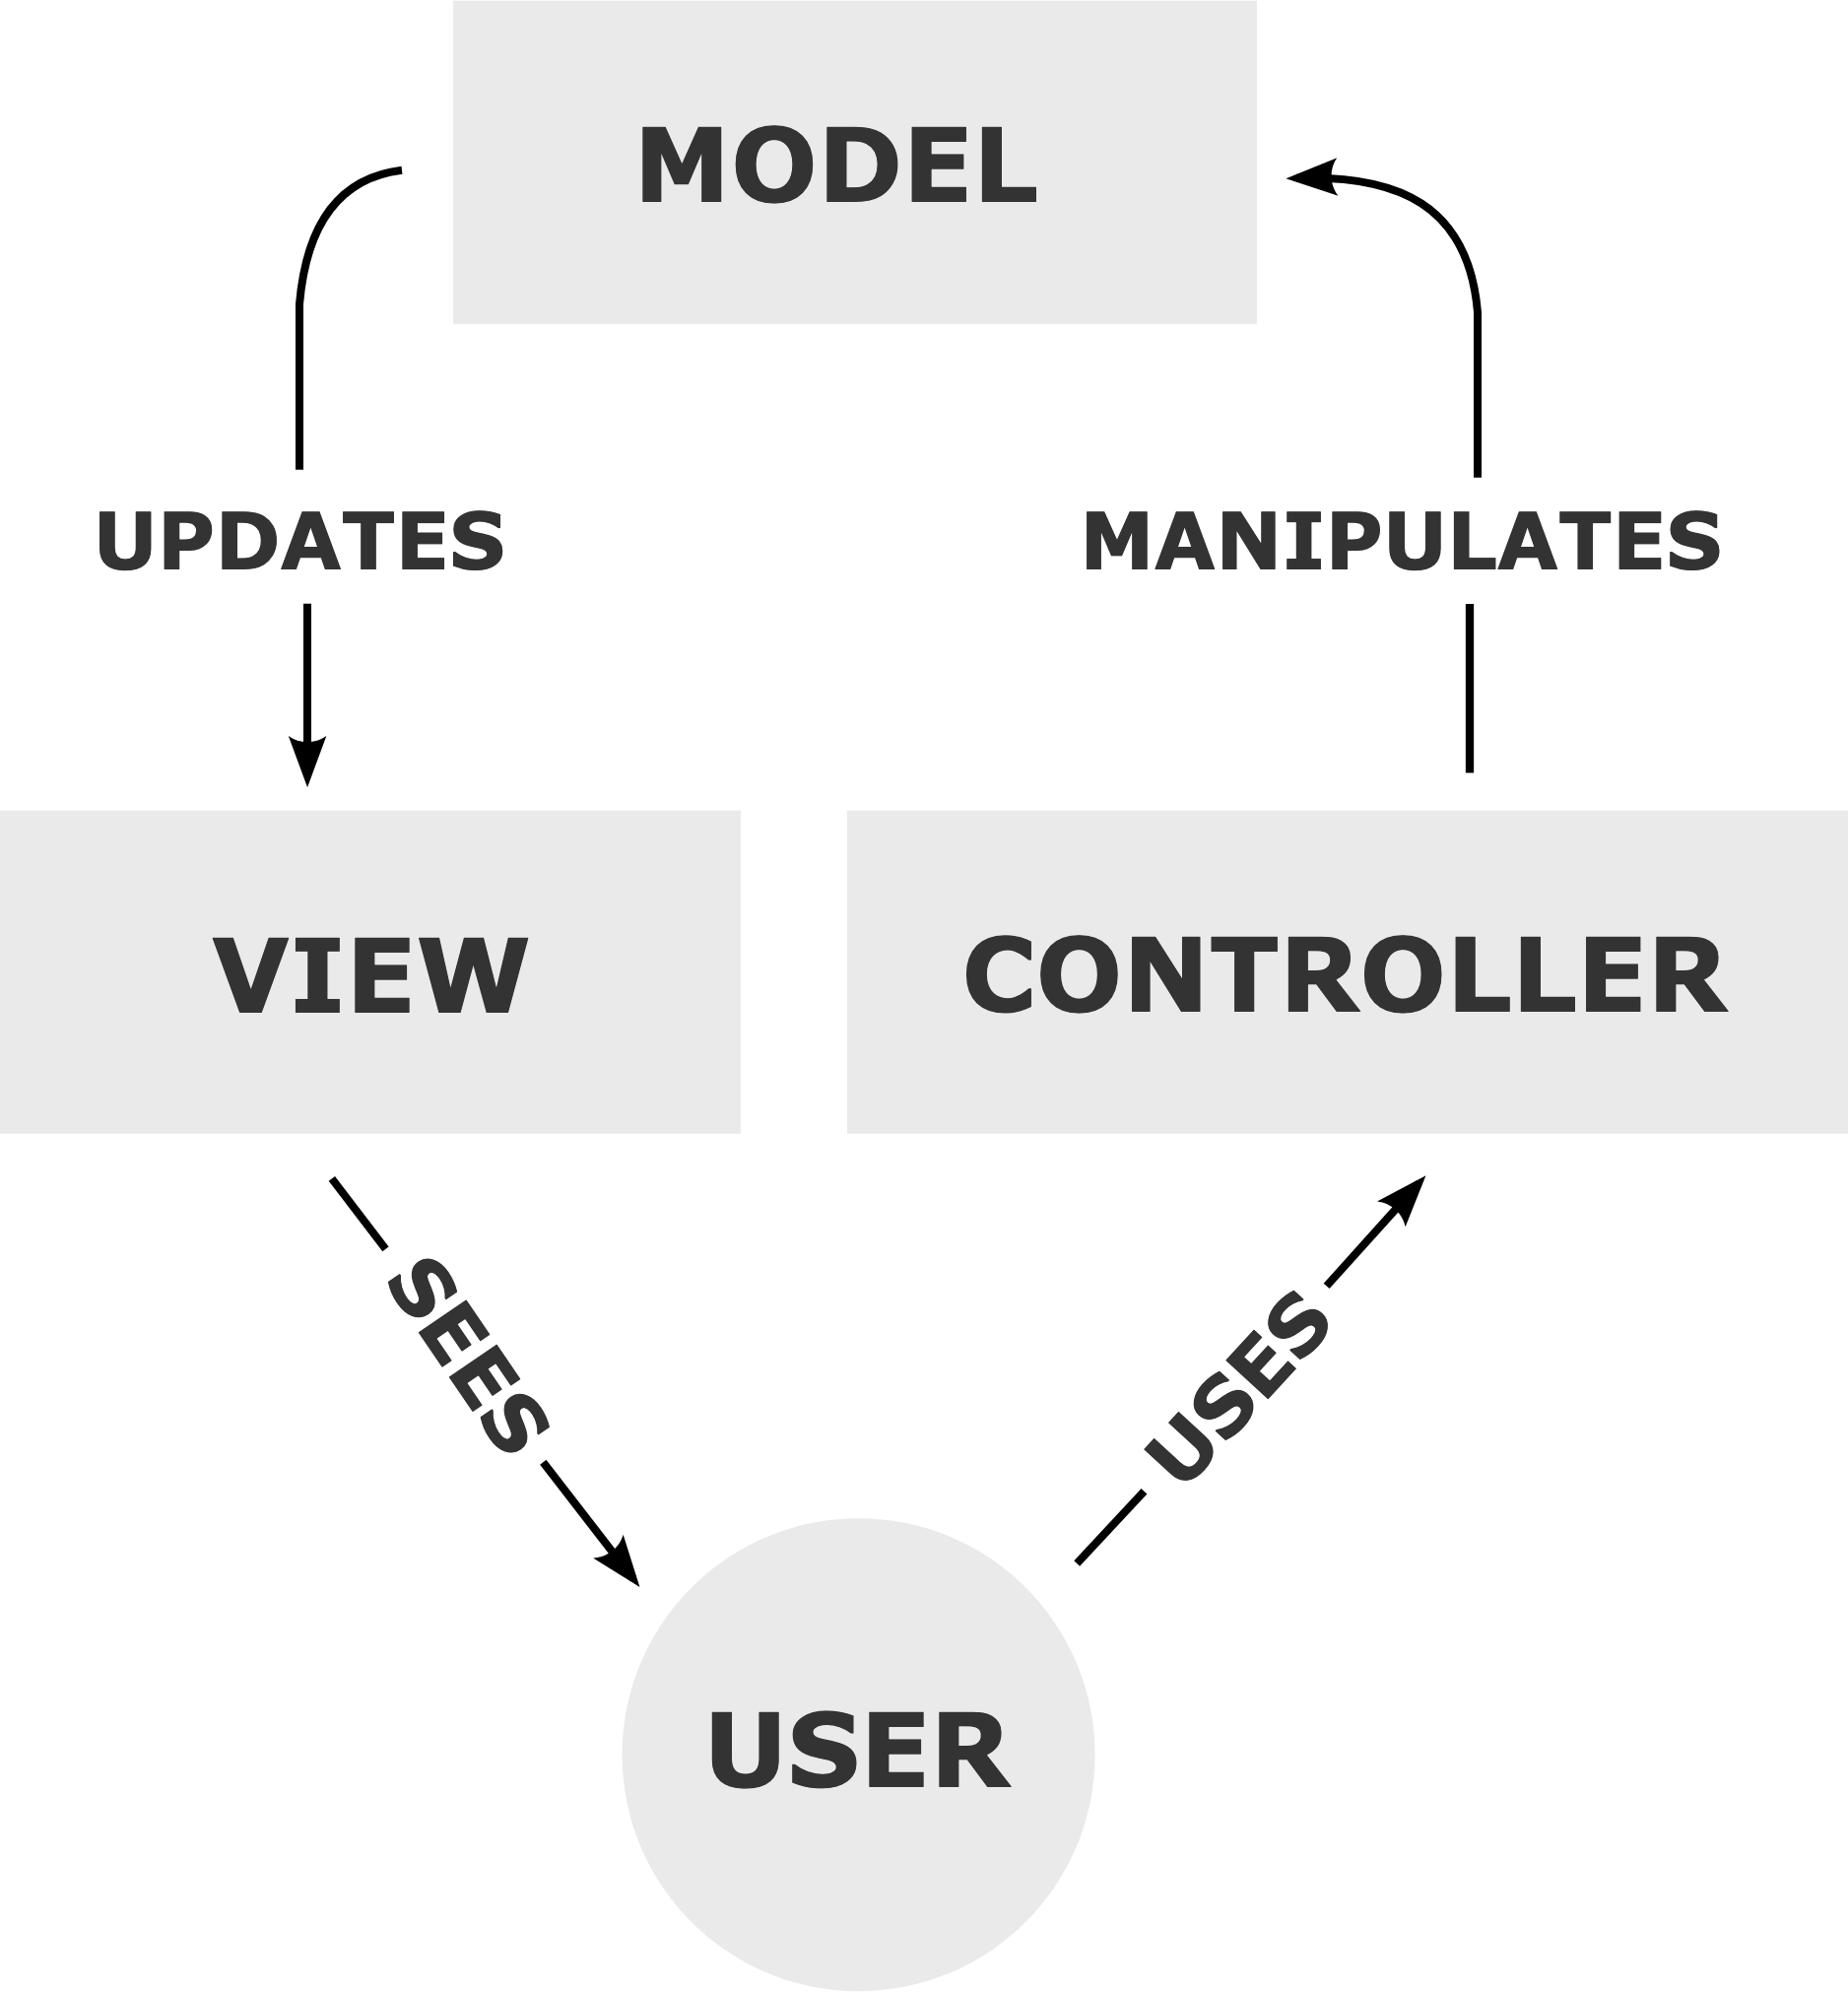
\includegraphics[scale=0.15]{assets/wikipedia_mvc_process}
\end{figure}

\color{red}

\subsubsection{Pattern X}
tbd

\subsubsection{Pattern Y}
tbd

\subsubsection{Pattern Z}
tbd

\color{black}
